\documentclass[11pt,letterpaper]{article}
\PassOptionsToPackage{hyphens}{url}
\usepackage[margin=.83in,top=.8in,bottom=.8in,headheight=15pt]{geometry}
\usepackage[T1]{fontenc}
\usepackage{lmodern,amsmath,amssymb,mathtools,bm,booktabs,array,graphicx,tikz}
\usetikzlibrary{arrows.meta,positioning,calc,decorations.pathreplacing,patterns}
\definecolor{ink}{HTML}{17344D}\definecolor{accent}{HTML}{087E8B}\definecolor{pale}{HTML}{EDF5F5}\definecolor{gold}{HTML}{AD6B19}
\providecommand{\dd}{\,\mathrm{d}}\providecommand{\R}{\mathbb{R}}
\providecommand{\E}{\mathbb{E}}\providecommand{\Var}{\operatorname{Var}}
\providecommand{\Cov}{\operatorname{Cov}}\providecommand{\diag}{\operatorname{diag}}
\providecommand{\norm}[1]{\left\lVert#1\right\rVert}
\providecommand{\abs}[1]{\left|#1\right|}
\usepackage{microtype,hyperref,fancyhdr,enumitem,amsthm,sectsty,needspace}
\allsectionsfont{\raggedright}
\hypersetup{colorlinks=true,linkcolor=ink,urlcolor=accent,pdfauthor={Zan Ahmad},pdftitle={Conservation of volume / Lecture notes}}
\setlength{\parindent}{0pt}\setlength{\parskip}{6pt}\linespread{1.07}
\setlist{itemsep=3pt,topsep=4pt,leftmargin=*}
\emergencystretch=2em\clubpenalty=10000\widowpenalty=10000
\pagestyle{fancy}\fancyhf{}\fancyhead[L]{\small Mathematical Modeling}\fancyhead[R]{\small Lecture 1}
\fancyfoot[L]{\footnotesize Zan Ahmad}\fancyfoot[R]{\footnotesize\thepage}\renewcommand{\headrulewidth}{.3pt}
\newtheorem{proposition}{Proposition}\newtheorem{theorem}{Theorem}\newtheorem{lemma}{Lemma}
\theoremstyle{definition}\newtheorem{definition}{Definition}\newtheorem{example}{Example}
\numberwithin{equation}{section}
\begin{document}
{\small\scshape Mathematical Modeling\hfill Lecture 1}\par\medskip
{\raggedright\hyphenpenalty=10000\exhyphenpenalty=10000\LARGE\bfseries\color{ink} Conservation of volume\par}\medskip
{\small Lecture notes}\par\bigskip
A model begins by specifying what can be measured and which transfers are retained. We shall derive a volume balance for a fixed boundary, solve it for a switched-flow experiment, and identify exactly when the prescribed experiment becomes physically impossible. The same cancellation argument will later conserve blood volume in a circulation network, population in an epidemic model, and charge exchanged by adjacent cable segments. The derivation uses an integral to add a changing rate over time; the derivative then expresses the same balance locally. Neither notation introduces a new physical assumption.

\section{A circulation diagram determines an accounting boundary}
\hypertarget{note-a-circulation-diagram-determines-an-accounting-boundary}{}\label{note:a-circulation-diagram-determines-an-accounting-boundary}
{\small \href{slides.html\#frame=compartment-volume-and-boundary-flux\&step=1}{Slides for this section}}\par
The adult circulation is a connected route: right heart, pulmonary vessels, left heart, systemic vessels, and back to the right heart. Arteries carry blood away from the heart and veins carry it toward the heart. These names do not specify oxygen content. Grouping many vessels into one compartment means that we retain their aggregate stored volume and their external connections, while discarding the internal distribution of that volume.

For the first calculation use a bench reservoir, with a fixed boundary, incompressible liquid, no evaporation, and no unrecorded leak. Define
\[
V(t)\quad[\mathrm{mL}],\qquad Q_{\mathrm{in}}(t),\ Q_{\mathrm{out}}(t)\quad[\mathrm{mL}/\mathrm{min}].
\]
Here the two flows are nonnegative magnitudes in their named directions. Time is measured in minutes. The flow functions are prescribed inputs: conservation determines storage from them, but does not explain which pump or pressure difference produces them. A pressure--flow law will be a separate model component in Meeting 2. One can therefore audit this first model without assuming a particular resistance or vessel geometry.

A statement of the question is also a statement of resolution. We ask how much fluid is present, not which fluid particle is present. Replacement of old fluid by new fluid can occur while the total volume is constant. Concentration and transit-time questions need additional states.
\begin{center}\begin{minipage}{.98\linewidth}\centering
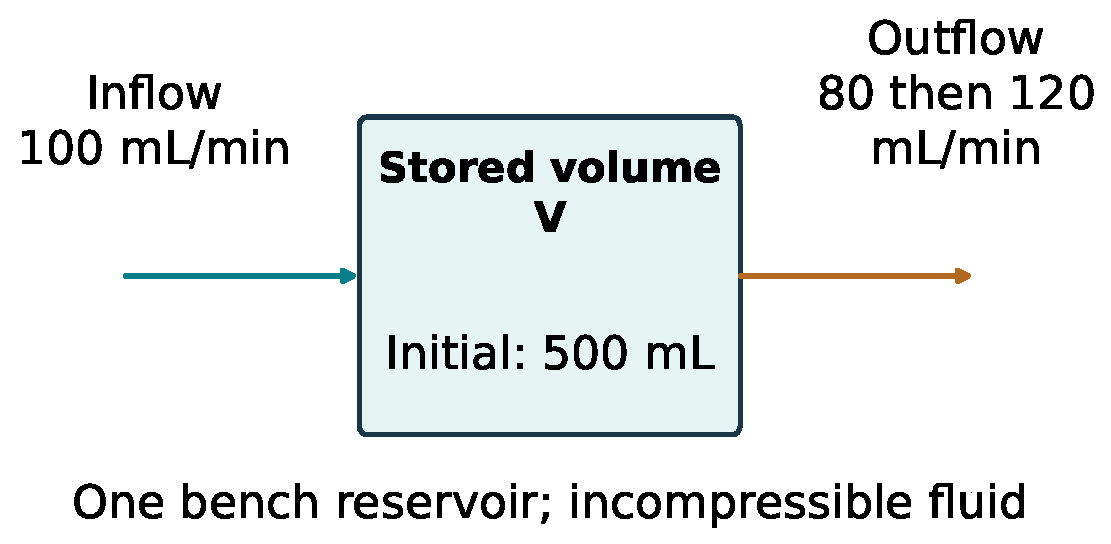
\includegraphics[width=.96\linewidth,height=.57\textheight,keepaspectratio]{presentation-figures/reservoir.pdf}\par\smallskip
{\small Original bench-reservoir model: volume is stored in mL; flows cross the boundary in mL/min. The outflow changes after three minutes.}
\end{minipage}\end{center}
\section{From transferred amounts to an integral balance}
\hypertarget{note-from-transferred-amounts-to-an-integral-balance}{}\label{note:from-transferred-amounts-to-an-integral-balance}
{\small \href{slides.html\#frame=add-small-transferred-amounts\&step=1}{Slides for this section}}\par
Let $t_0<t_1$. Divide the interval into small pieces of duration $\Delta t_k$. If the flow varies little on a piece, its incoming amount is approximately $Q_{\mathrm{in}}(t_k)\Delta t_k$. Adding pieces and taking a limit gives the cumulative input
\[
A_{\mathrm{in}}(t_0,t_1)=\int_{t_0}^{t_1}Q_{\mathrm{in}}(s)\,ds,
\qquad
A_{\mathrm{out}}(t_0,t_1)=\int_{t_0}^{t_1}Q_{\mathrm{out}}(s)\,ds.
\]
The letter $s$ is an integration variable; it is not a second physical clock. Conservation says
\[
\boxed{V(t_1)-V(t_0)=\int_{t_0}^{t_1}\bigl[Q_{\mathrm{in}}(s)-Q_{\mathrm{out}}(s)\bigr]\,\dd s.}
\]
Every term is a volume. In particular, $[Q\,ds]=(\mathrm{mL}/\mathrm{min})\mathrm{min}=\mathrm{mL}$. At $100\ \mathrm{mL}/\mathrm{min}$, thirty seconds transfers $100(30/60)=50\ \mathrm{mL}$.

Where the inputs are continuous, divide the balance over $[t,t+h]$ by $h$ and let $h\to0$:
\[
\frac{dV}{dt}=Q_{\mathrm{in}}(t)-Q_{\mathrm{out}}(t),\qquad V(t_0)=V_0.
\]
The differential equation and initial condition determine a trajectory. The integral balance remains valid even at a finite jump in the prescribed rate. Such a jump changes the slope of $V$, not $V$ itself; an instantaneous volume jump would require an impulsive transfer, which is absent here.
\Needspace{10\baselineskip}
\section{An exact switched-flow experiment}
\hypertarget{note-an-exact-switched-flow-experiment}{}\label{note:an-exact-switched-flow-experiment}
{\small \href{slides.html\#frame=first-constant-flow-interval\&step=1}{Slides for this section}}\par
Take $V_0=500\ \mathrm{mL}$, a constant inflow $Q_{\mathrm{in}}=100\ \mathrm{mL}/\mathrm{min}$, and
\[
Q_{\mathrm{out}}(t)=
\begin{cases}80,&0\leq t<3,\\120,&3\leq t\leq6,
\end{cases}
\qquad [\mathrm{mL}/\mathrm{min}].
\]
The exact solution is obtained one interval at a time:
\[
V(t)=\begin{cases}
500+20t,&0\leq t\leq3,\\
560-20(t-3),&3\leq t\leq6.
\end{cases}
\]
The second interval starts from the first interval's endpoint, not from the original initial condition. Thus $V(3)=560$ and $V(6)=500\ \mathrm{mL}$. The cumulative account is
\[
A_{\mathrm{in}}(0,6)=100(6)=600,\qquad
A_{\mathrm{out}}(0,6)=80(3)+120(3)=600\quad[\mathrm{mL}].
\]
Equal initial and final volumes do not imply zero flow between them. Nor do they determine the intermediate volume: the time-resolved inputs are needed for that.

The upper plot shows inputs; the lower plot shows their integral consequence. A straight volume segment identifies a constant net rate. A horizontal segment requires equal inflow and outflow, which could both be zero or both be large. At $t=3$, the slopes on the two sides are $+20$ and $-20\ \mathrm{mL}/\mathrm{min}$. The corner records the switching idealization.
\begin{center}\begin{minipage}{.98\linewidth}\centering
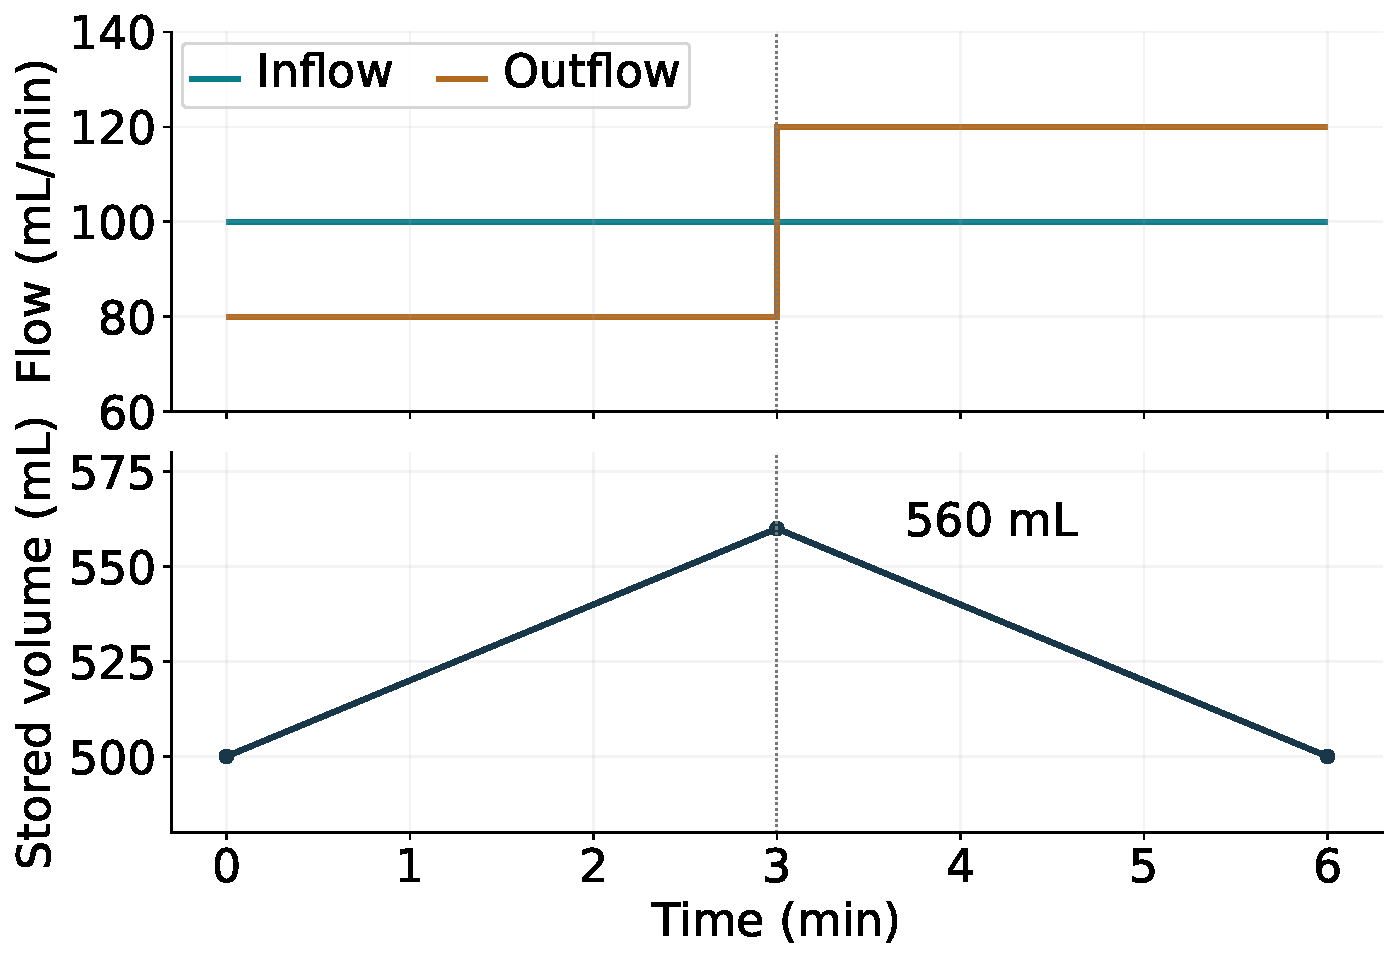
\includegraphics[width=.96\linewidth,height=.57\textheight,keepaspectratio]{presentation-figures/flow-and-storage.pdf}\par\smallskip
{\small Exact interval accounting for synthetic piecewise constant flows. At minute 3 the flow changes while stored volume stays continuous.}
\end{minipage}\end{center}
\section{Why internal transfers disappear from a larger balance}
\hypertarget{note-why-internal-transfers-disappear-from-a-larger-balance}{}\label{note:why-internal-transfers-disappear-from-a-larger-balance}
{\small \href{slides.html\#frame=enlarge-the-boundary\&step=1}{Slides for this section}}\par
Consider two reservoirs. Let $q(t)$ be the signed flow from reservoir 1 to reservoir 2, $a(t)$ an external input to reservoir 1, and $b(t)$ an external output from reservoir 2. Their balances are
\[
\frac{dV_1}{dt}=a-q,\qquad \frac{dV_2}{dt}=q-b.
\]
Adding gives $d(V_1+V_2)/dt=a-b$. The value of $q$ need not be zero or constant. Cancellation follows because the very same transfer occurs once with each sign.

More generally, orient every link in a network and form its incidence matrix $B$: column $e$ has $-1$ at the source of link $e$ and $+1$ at its destination. With stored-volume vector $\mathbf V$, link-flow vector $\mathbf Q$, and external source vector $\mathbf u$,
\[
\dot{\mathbf V}=B\mathbf Q+\mathbf u,
\qquad \mathbf1^{T}B=0,
\qquad
\frac{d}{dt}\mathbf1^{T}\mathbf V=\mathbf1^{T}\mathbf u.
\]
This is the same elementary account in matrix notation. A closed circulation has $\mathbf u=0$, so its total volume is invariant even while all component volumes vary. An implementation that calculates two different values for one shared flow breaks the cancellation.
\section{Admissibility and the emptying event}
\hypertarget{note-admissibility-and-the-emptying-event}{}\label{note:admissibility-and-the-emptying-event}
{\small \href{slides.html\#frame=locate-the-first-impossible-continuation\&step=1}{Slides for this section}}\par
For a constant interval starting at time $t_k$, write $r_k=Q_{\mathrm{in},k}-Q_{\mathrm{out},k}$ and $V(t_k+s)=V_k+r_ks$. If $r_k<0$, the first emptying time is
\[
\tau_k=\frac{V_k}{-r_k}.
\]
The interval is physically admissible only while $0\leq s\leq\tau_k$. Because a linear segment attains its minimum at an endpoint, checking both endpoint volumes is sufficient on a constant-rate interval. For example, $V_k=50\ \mathrm{mL}$ and net removal $20\ \mathrm{mL}/\mathrm{min}$ imply emptying after $2.5\ \mathrm{min}$.

Continuing the same rule beyond that event gives negative storage. Clipping that result to zero silently adds fluid to the account. Instead stop the calculation at the event, or replace the prescribed outflow with a justified state-dependent law. This separates a correct solution of the stated equations from the physical admissibility of those equations.

If characteristic volume and flow are $V_c$ and $Q_c>0$, the ratio $T_c=V_c/Q_c$ has units of time. It is an accumulation scale. It is an emptying time only when the actual net removal equals the chosen constant $Q_c$; a ratio of units does not by itself establish a mechanism.
\section{Exact interval updates and evidence for the model}
\hypertarget{note-exact-interval-updates-and-evidence-for-the-model}{}\label{note:exact-interval-updates-and-evidence-for-the-model}
{\small \href{slides.html\#frame=an-exact-interval-algorithm\&step=1}{Slides for this section}}\par
For piecewise constant inputs the program uses
\[
V_{k+1}=V_k+(Q_{\mathrm{in},k}-Q_{\mathrm{out},k})\Delta t_k.
\]
This is exact integration of the specified input on each interval, not an approximation obtained merely by making a numerical step small. Its accumulated residual should satisfy
\[
\mathcal R_k=V_k-V_0-
\sum_{j<k}(Q_{\mathrm{in},j}-Q_{\mathrm{out},j})\Delta t_j=0
\]
up to floating-point roundoff. Independently check zero flow, equal nonzero flows, splitting an interval without changing its rates, and a consistent conversion from mL to L. These tests exercise the intended account.

A model test uses independently measured flows to predict independently measured volumes. If $V^{\mathrm{obs}}(t)$ is the measured volume, inspect $V^{\mathrm{obs}}(t)-V^{\mathrm{pred}}(t)$ through time rather than only at the endpoint. A persistent discrepancy can indicate a missing connection, a biased flow sensor, or an inadequate prescribed-input approximation. A numerical residual close to zero cannot distinguish these possibilities: it verifies the internal account, not the physical assumptions.
\bigskip
\section*{Exercises}
\par\noindent\begin{minipage}{\linewidth}
\subsection*{M1-1. Account for a transfer}
A reservoir starts with 300 mL. Inflow is 50 mL/min and outflow is 35 mL/min for 4 minutes.

\textbf{a} Calculate the amount entering and leaving.

\end{minipage}\par\medskip
\textbf{b} Find final storage and state the independent budget equality.

\textbf{c} Would the same final storage prove that no fluid moved? Explain.

\par\noindent\begin{minipage}{\linewidth}
\subsection*{M1-2. Repair a unit mismatch}
A flow meter reads 120 mL/min. The collection lasts 30 seconds.

\textbf{a} Convert the interval to minutes and calculate collected volume.

\end{minipage}\par\medskip
\textbf{b} A program multiplies 120 by 30 and reports 3600 mL. Identify the mistake.

\textbf{c} Express the correct result in liters and give one useful check.

\par\noindent\begin{minipage}{\linewidth}
\subsection*{M1-3. Move the boundary}
Two reservoirs A and B begin with 200 mL each. An external 50 mL/min enters A; 30 mL/min moves from A to B; 20 mL/min leaves B to the outside. Rates stay fixed for 2 minutes.

\textbf{a} Calculate the final volume in each reservoir.

\end{minipage}\par\medskip
\textbf{b} Compute the combined final volume without using the internal transfer.

\textbf{c} Explain why the two methods agree.

\par\noindent\begin{minipage}{\linewidth}
\subsection*{M1-4. Detect an impossible continuation}
A reservoir has 60 mL, no inflow, and a prescribed outflow of 20 mL/min.

\textbf{a} When would it empty under the constant-flow assumption?

\end{minipage}\par\medskip
\textbf{b} What does the same rule predict after 4 minutes, and why is that unacceptable?

\textbf{c} Propose a defensible model revision and one observation that would help choose it.

\section*{References}
\noindent\begin{minipage}{\linewidth}
Zan Ahmad, Fall 2024 HEART syllabus. PDF pages 1--2.

\end{minipage}\par\medskip
\noindent\begin{minipage}{\linewidth}
Hoppensteadt and Peskin, Modeling and Simulation in Medicine and the Life Sciences, second edition. Printed pages 5--8; PDF pages 18--21 in the supplied copy.

\end{minipage}\par\medskip
\end{document}
